\chapter{Versuch 2}
\label{chap:VERSUCH_2}

\section{Fragestellung, Messprinzip, Aufbau, Messmittel}
\label{chap:VERSUCH_2_FRAGESTELLUNG}
\subsection*{Fragestellung}
Im 2 Versuch geht es darum durch die Aufnahme eines Dunkelbilds Pixel zu finden, die trotz kompletter Dunkelheit nicht den Wert 0(aus) zurück liefern.
\subsection*{Messprinzip}
Durch diesen Versuch werden die sogenannten Hot / Stuck Pixel erkannt(die Pixel die nicht 0 zurück liefern). Diese werden unter anderem durch das thermische Rauschen der Ausleseelektronik verursacht wird.
\subsection*{Aufbau}
Die Kamera wird vollständig verdunkelt zum Beispiel durch einen Aufkleber vor der Linse.
\subsection*{Messmittel}
Wie bei Versuch 1

\newpage
\section{Messwerte}
\label{chap:VERSUCH_2_MESSWERTE}
Es werden 10 Dunkelbild aufnahmen gemacht und in Grauwertbilder umgerechnet:
\linebreak
\begin{tabular}{ccccc}

\includegraphics[scale=0.1]{media/dunkelbilder/dunkelbild_0} & 
\includegraphics[scale=0.1]{media/dunkelbilder/dunkelbild_1} & 
\includegraphics[scale=0.1]{media/dunkelbilder/dunkelbild_2} & 
\includegraphics[scale=0.1]{media/dunkelbilder/dunkelbild_3} & 
\includegraphics[scale=0.1]{media/dunkelbilder/dunkelbild_4} \\ 

\includegraphics[scale=0.1]{media/dunkelbilder/dunkelbild_5} & 
\includegraphics[scale=0.1]{media/dunkelbilder/dunkelbild_6} & 
\includegraphics[scale=0.1]{media/dunkelbilder/dunkelbild_7} & 
\includegraphics[scale=0.1]{media/dunkelbilder/dunkelbild_8} & 

\includegraphics[scale=0.1]{media/dunkelbilder/dunkelbild_9} \\ 
\end{tabular} 


\section{Auswertung}
\label{chap:VERSUCH_2_AUSWERTUNG}
Aus den 10 Dunkelbild Aufnahmen wird dann der pixelweise Mittelwert berechnet und ein neues Dunkelbild erzeugt. Dies soll das thermische Ausleserauschen eliminieren und es bleibt nur noch der Offset jedes Pixels übrig:


\includegraphics[scale=0.4]{media/dunkelMean}

Auf dem ersten Blick sieht man nicht sehr viel. Allerdings wenn man das Dunkelbild Kontrast maximiert darstellt ergibt sich folgendes:

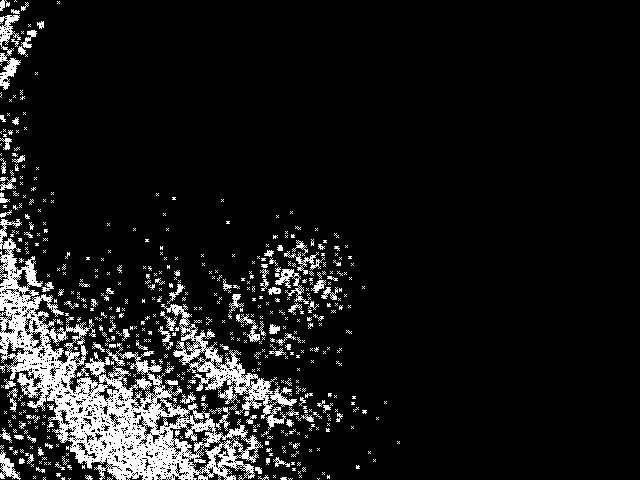
\includegraphics[scale=0.4]{media/dunkelContrastMax}

Jetzt wird jeder Pixel der aufgrund des thermischen Rauschens nicht den Wert 0 hat Kontrast maximiert dargestellt in weiß.

\section{Interpretation}
\label{chap:VERSUCH_2_INTERPRETATION}
Aus dem Kontrast maximierten Bild kann man sehr gut erkennen wie stark das Rauschen sein kann. Im Zusammenhang mit einer nicht sehr neuen Kamera die in diesem Fall verwendet wurde, ist das thermische Rauschen mit hoher Wahrscheinlichkeit viel stärker als bei neueren Kameras. 